\chapter{Approach}
% TODO: remember to justify the choices made
% also compare different possibilities

In this chapter, the work towards modeling a moving human is described. Starting out, there was much to be figured out and tried. Many questions were not only unanswered but still unasked. The target was already defined: a rigged 3D mesh of the user. The tools available were a Microsoft Kinect for Xbox 360 and a desktop computer.

\section{Obtaining point cloud data}

The first step towards achieving anything with a Kinect is, obviously, to read its sensor data to the computer. This is not trivially easy considering that Kinect was originally only meant to be an Xbox 360 accessory. When the work on this thesis began, at least three different drivers for Kinect were available. Each of them were installed and tested by writing trivial software using them.

\fixme{are these appropriate in here, or should some parts be moved to Related Work?}

\subsection{Microsoft Kinect SDK}

The obvious solution for developing software that uses Kinect is the Microsoft Kinect for Windows Software Development Kit (SDK)\footnote{The Microsoft Kinect SDK is available at \url{http://www.microsoft.com/en-us/kinectforwindows/}.}. Kinect is a Microsoft product, so Microsoft will surely supply the SDK, right? This wasn't true to begin with, and Microsoft actually only released the SDK after open-source drivers had gained momentum.

The Microsoft SDK is available for Windows 7 and later. It supports development in C++/CLI, C\# or Visual Basic .NET. A multitude of features have been included in the SDK. For example, skeleton tracking, face tracking and audio input are supported.

License restrictions in the Microsoft Kinect SDK make it unappealing. For example, using a Microsoft Kinect for Xbox 360 is allowed for development, but distributing created software for use with it is forbidden. Only using a Microsoft Kinect for Windows sensor is allowed for end-users. This is required to be ``clearly stated'' in all materials related to any created application. Moreover, the end-user license agreement (EULA) forbids applying a copyleft license to applications created using the Microsoft SDK. \citep{kinectEULA}

Skeleton tracking using the Microsoft SDK was tested by compiling a sample application and making modifications to it. The API seems to be good and usable, and the skeleton tracking methods work quite well. Fast movement and occlusion caused problems such as the skeleton jumping into weird poses for a short time.

\subsection{OpenKinect}

OpenKinect\footnote{\url{http://openkinect.org/}} is an open community project aiming at creating open-source software for using Kinect. The main focus of the project is the libfreenect library, available under the terms of Apache License 2.0 \citep{Apache2} or the GNU General Public License (GPL) 2.0 \citep{GPL2}.

OpenKinect is made from scratch by hobbyists, and remains very low-level. It is possible to read video and depth data, but combining them to create point clouds is not supported by libfreenect. \citet{burrus2010} shows a workable calibration procedure, and also shares the measured calibration parameters for others to use. \citet{fisher2010} shows example code of using these parameters to transform video and depth images to colored points in world coordinates.

Tilting the Kinect using the built-in motor and changing the color of the led are also supported by libfreenect. While not particularly useful in most applications, these features are notable as they are missing from OpenNI, the other freely available driver.

Of the three drivers, libfreenect was the easiest to start working with. By installing the OpenKinect plugin for Processing \citep{shiffman2010}, the Kinect was up and running in minutes. Development was easy given the bundled examples, which include creating point clouds as shown by \citet{fisher2010}. Apparently the functionality is still quite low-level, and thus not very suitable for trying to capture human body details.

\subsection{OpenNI}

The OpenNI (Open Natural Interaction) library \citep{OpenNI} is developed by PrimeSense, which also manufactures the sensor hardware used in Microsoft Kinect and the Asus Xtion series. OpenNI is available under the GNU Lesser General Public License (LGPL), version 3 \citep{LGPL3}.

OpenNI supports embedding middleware that can greatly enhance functionality of the library. PrimeSense leverage this architecture by supplying a proprietary middleware called NITE\footnote{NITE seems to be an acronym, but its meaning is not commonly disclosed.} \citep{NITE}. 

OpenNI was finally chosen to be used for data acquisition in this work.

\section{Experiments with point clouds}

\begin{figure}
    \centering
    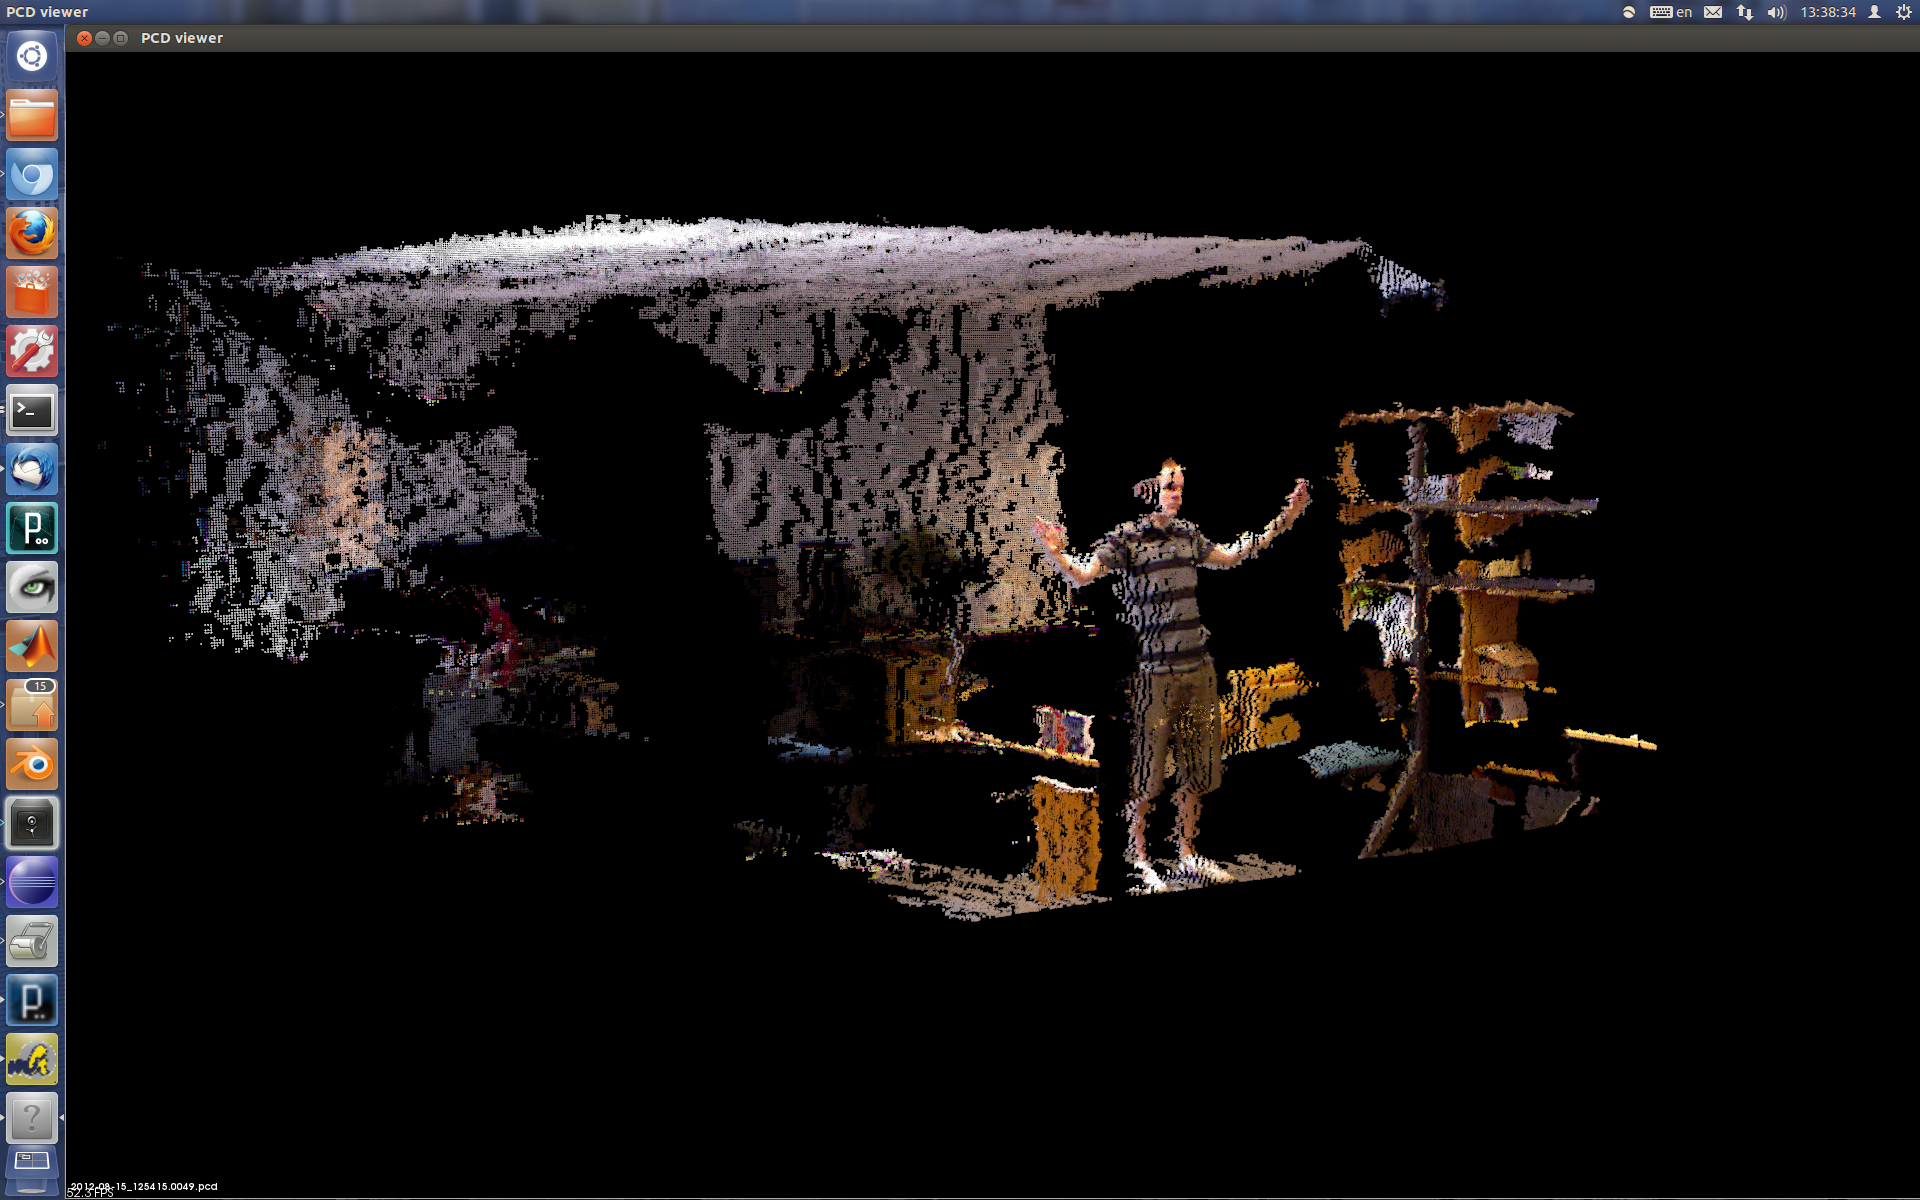
\includegraphics[width=\textwidth]{pcd-plain.png}
    \caption{A point cloud constructed from a single frame of Kinect data. The cloud is captured and saved in the .pcf format (Point Cloud Format) that PCL uses. The viewer used is part of PCL.}
    \label{fig:pcd-plain}
\end{figure}

\section{Body part segmentation}

Before any attempts at human body reconstruction can be made, the body needs to be detected from the RGB-D image. % mention 'segmentation'

The NITE middleware for OpenNI \citep{NITE}
includes functions for person detection. Moreover, NITE has the capability to generate a skeleton representation of human users.

As the skeleton representation is available, we used it to aid in reconstructing the body model.

Using the skeleton data, we segment the point cloud according to body parts.

\fixme{The body parts used were chosen according to what the NITE skeleton allowed.} Thus the following segments were used:

\fixme{TODO: what do we really have? what are the right English terms?
legs, feet, forearms, shoulders, head, torso, hip}

\begin{figure}
    \centering
    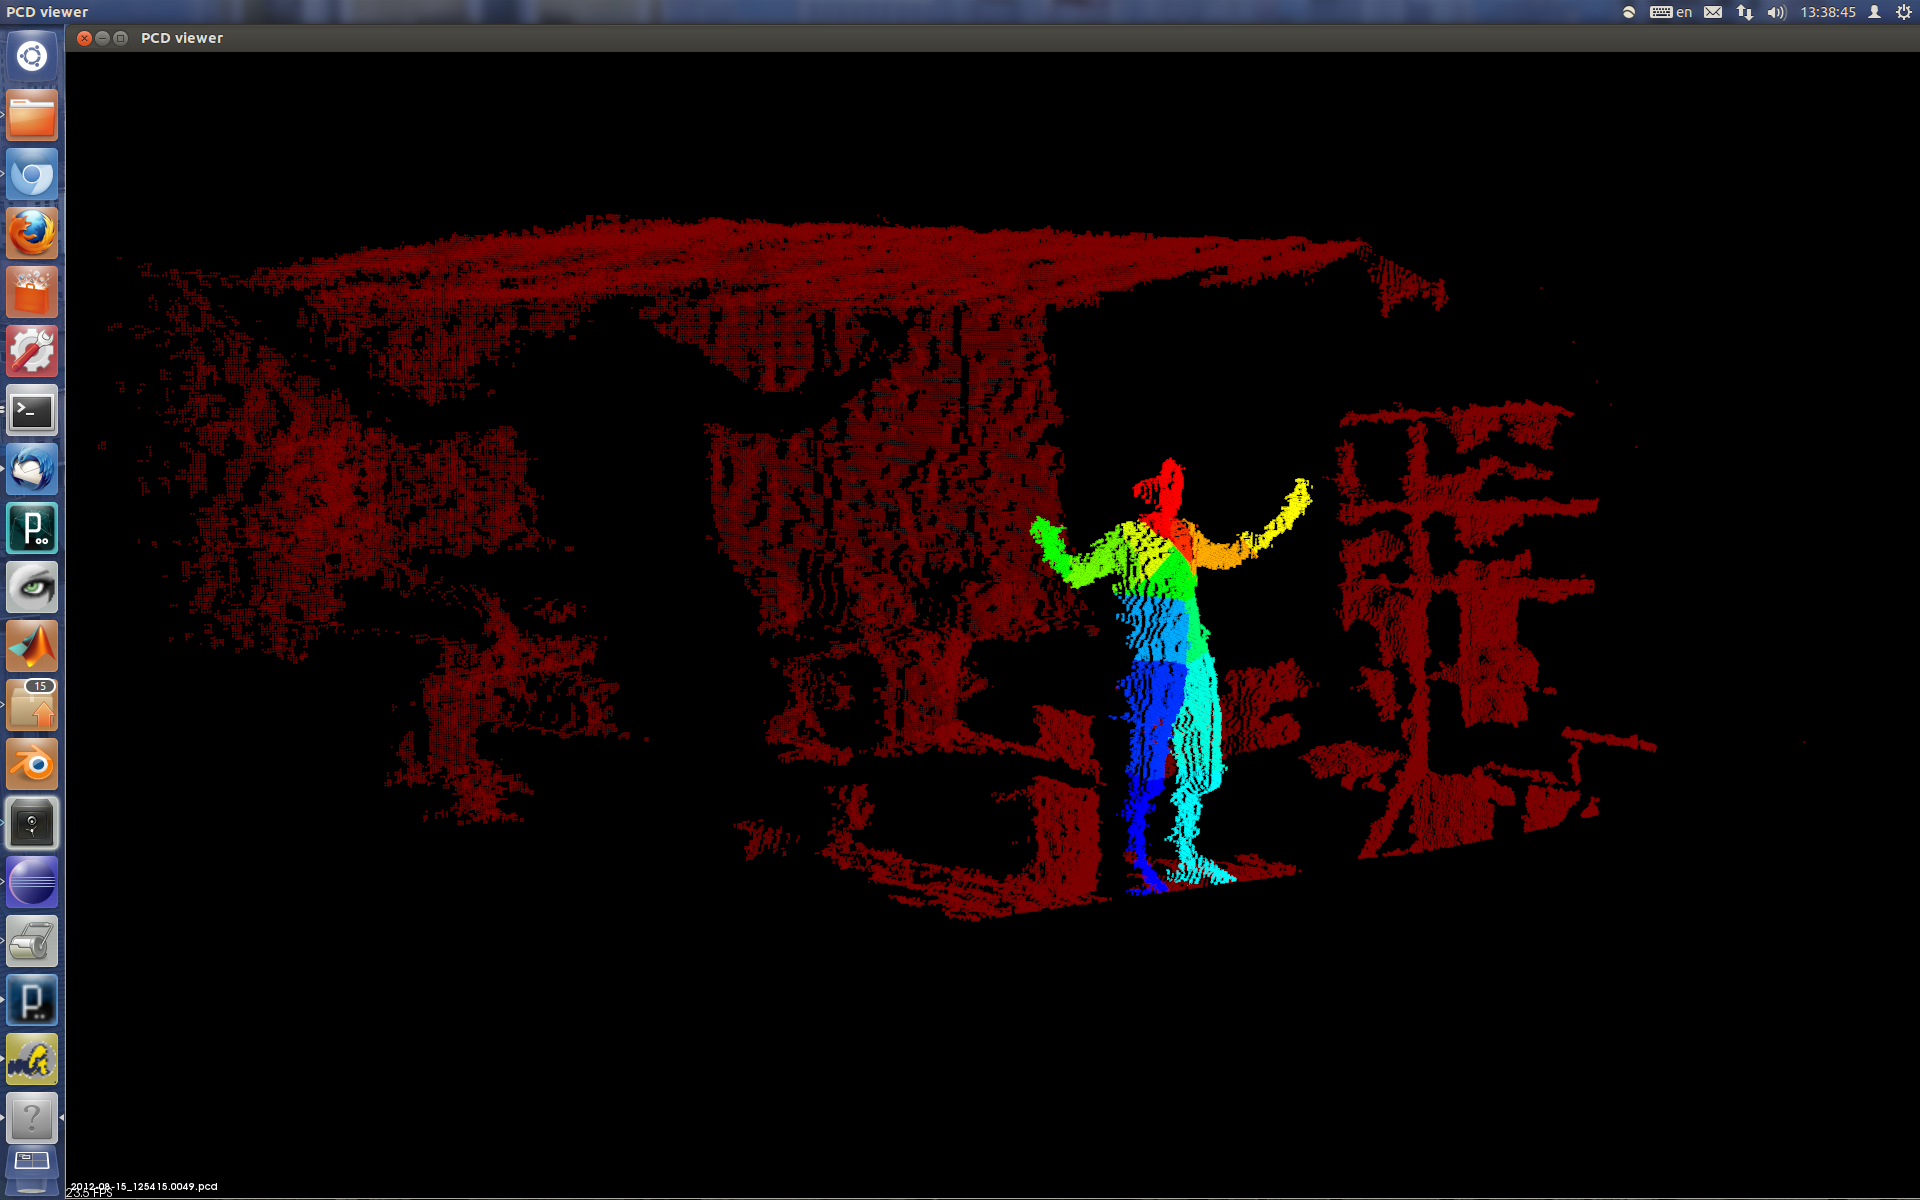
\includegraphics[width=\textwidth]{pcd-segmented.png}
    \caption{The same point cloud as in \ref{fig:pcd-plain}, with user segmented from the background, and further segmented into individual body parts.}
    \label{fig:pcd-segmented}
\end{figure}

\section{Point cloud alignment}

The naïve approach to modeling uses data only from a single frame. However, this is unsatisfactory as in practice only less than a half (e.g. the front part) of a human can be seen at once. Another consideration is that the data tends to be noisy and inaccurate. Accumulating data over time makes it possible to remove some of the noise and improve accuracy.

To allow for combining data from multiple frames, the observations (point clouds) need to be aligned one way or another. Methods introduced in \autoref{literature.alignment} were available, each with their own trade-offs.

\fixme{write more about this when the best approach is actually chosen}

\section{Mesh generation}

\fixme{Alternative approaches, including the following}

\subsection{Voxel grid}

One possible approach is to use a voxel grid similar to the one Kinect Fusion \citep{} uses. This allows generating meshes representing arbitrary shapes.

To evaluate the approach, a prototype was built on top of Kinfu\footnote{Kinfu is an open source implementation of Kinect Fusion \citep{newcombe2011kinectfusion}. It is included in the Point Cloud Library \citep{PCL}.}. Since the point clouds were already segmented by body part, it was possible to create recordings that only include a single body part. These recordings could then be played back and used as input for Kinfu.

The working hypothesis was that each body part could be treated as a static object, and that Kinfu should do quite well at modeling them. \fixme{Notably there's little difference between the camera moving} (as is the case in Kinect Fusion) and the object moving. If the background is filtered out, the result is similar. This made for the case that running the Kinect Fusion algorithm in parallel to each body part could give reasonably good results.

In practice, Kinfu doesn't work well with isolated limb data. This has multiple causes. \fixme{1) For full-body scanning the whole user must obviously fit in the picture. At the VGA resolution that Kinect uses, this leaves few pixels per limb. 2) The depth resolution of Kinect is about 1--2 centimeters at a distance suitable for full-body scanning. 3) ICP only uses surface features for alignment, not color data. As the individual body parts tend to be quite smooth, this is a problem.}

% TODO: split into three different images
\begin{figure}
    \centering
    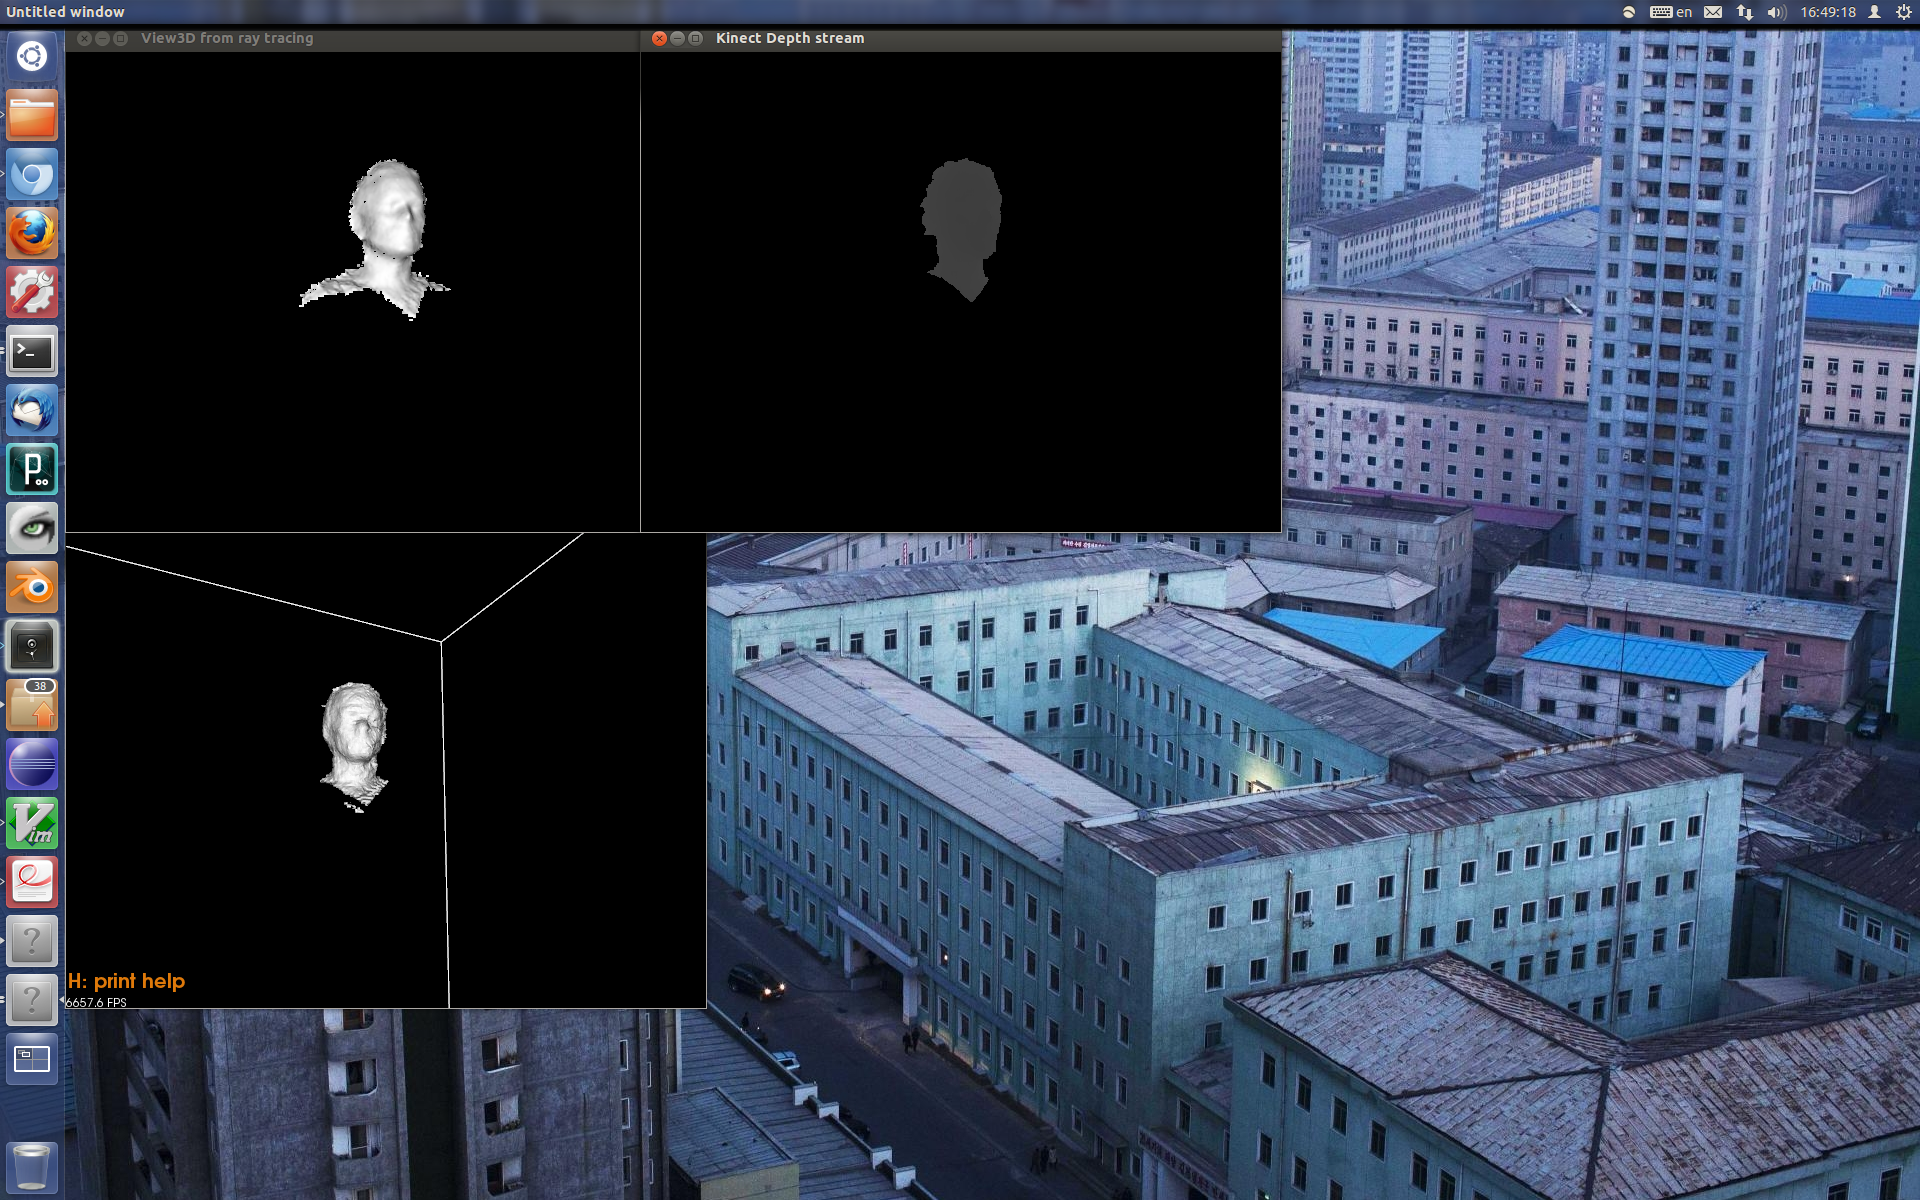
\includegraphics[width=\textwidth]{limbwise-head.png}
    \caption{Kinfu running on a view with only the head.}
    \label{fig:limbwise-head}
\end{figure}

% TODO: split into three different images
\begin{figure}
    \centering
    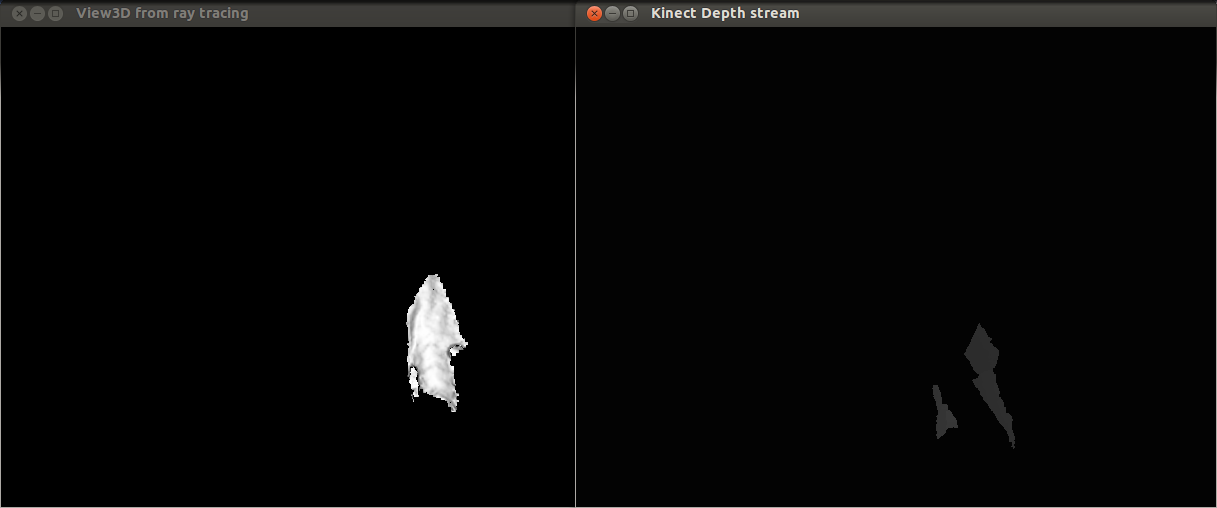
\includegraphics[width=\textwidth]{limbwise-arm.png}
    \caption{Kinfu running on a view with only the left arm.}
    \label{fig:limbwise-arm}
\end{figure}

\subsection{Parametric surfaces}

Another approach is to use the information readily available about the body parts being modeled. Instead of allowing arbitrary shapes, the space of possible shapes can be limited to what the body parts tend to look like.

As the very first prototype, a simple cylinder approximation was used. A cylinder was fitted to the point cloud of a body part, and colored according to its average color. This was good for testing the segmentation and getting a general idea of how accurate the skeleton is. Some corner cases were also found using this prototype. \fixme{elaborate...} \fixme{TODO: screenshot}

Obviously, a more human-like model was needed. The "cylinder man" could be usable as an avatar, and is certainly recognizable as human-like. But certainly its shape was nowhere near a real human body. Different simple shapes such as ellipsoids were considered. This would still have left the problem of connecting the body parts. Some kind of a meta-blob solution might have been feasible, but in the end this approach started to seem quite cumbersome. And still the accuracy would have left much to be hoped for.

The best parametric model for the purpose would then be something that already assumes the generic human shape, while allowing \fixme{exact} modifications to single body parts. The SCAPE model \citep{anguelov2005scape} used by \citet{weiss2011home} fits the description, but is not suitable for real-time evaluation. A more suitable approach is taken by MakeHuman \citep{makehuman}, which uses a base mesh and has defined parameters that can be used to reshape different parts of the mesh.

MakeHuman is still in development and at the time of writing was undergoing some large changes. It is not designed to be used as a library, either. Interfacing with other software thus seemed nontrivial. After some time tinkering with the MakeHuman implementation, it was decided that the data is important while the software can be replaced. The most important features were not very difficult to implement.

\fixme{Where should the implementation details of MakeHuman be described?}

\begin{figure}
    \centering
    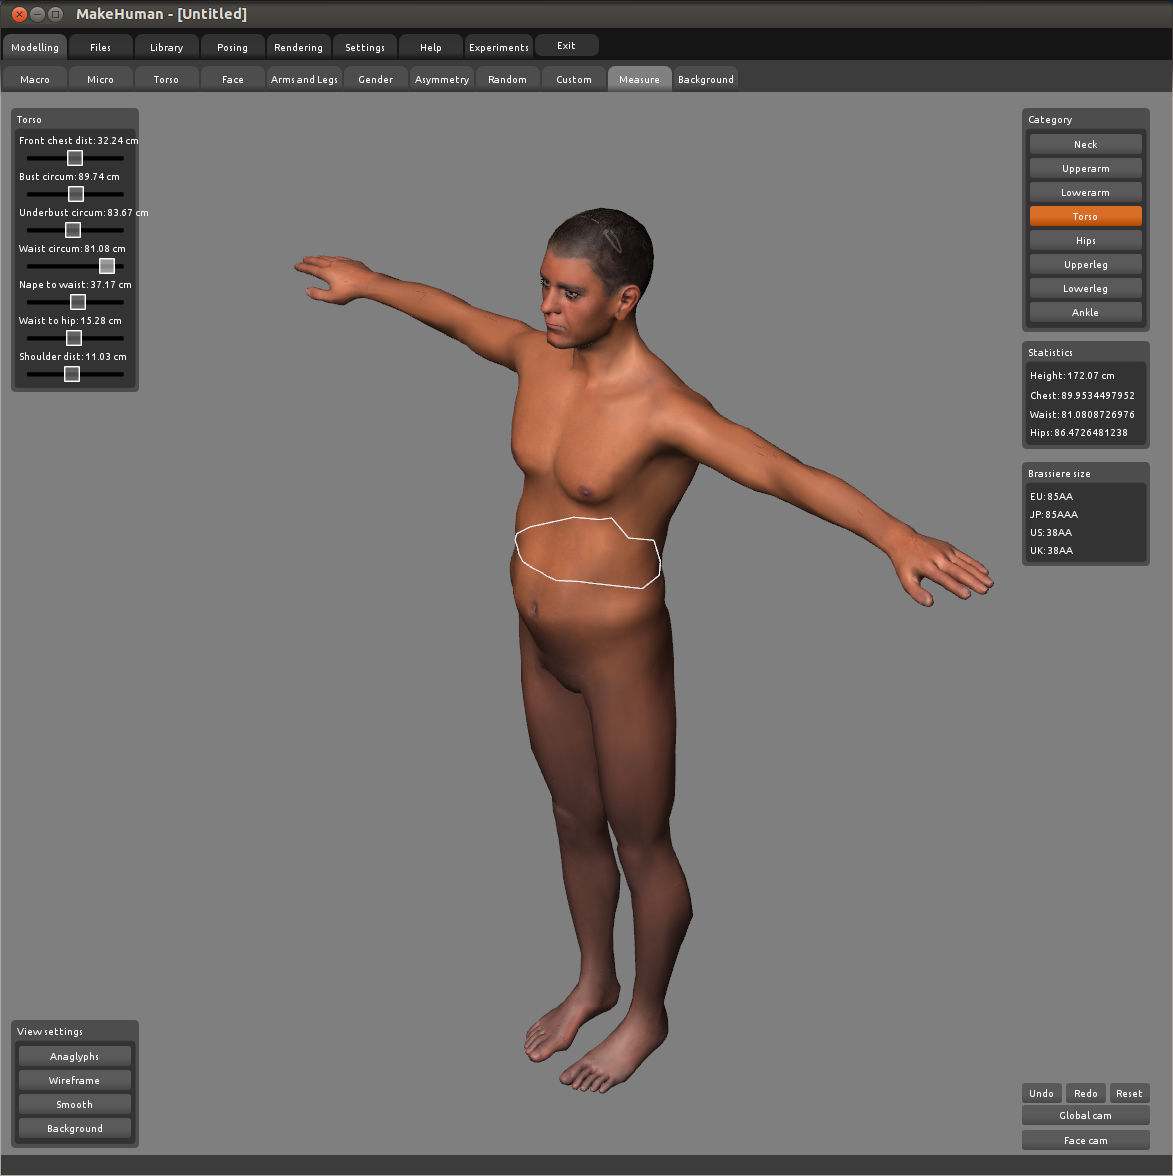
\includegraphics[width=\textwidth]{makehuman-measurement.png}
    \caption{MakeHuman with the Measurement plugin active. Waist circumference is selected. The white line shows where the circumference is measured.}
    \label{fig:makehuman-measurement}
\end{figure}

\begin{figure}
    \centering
    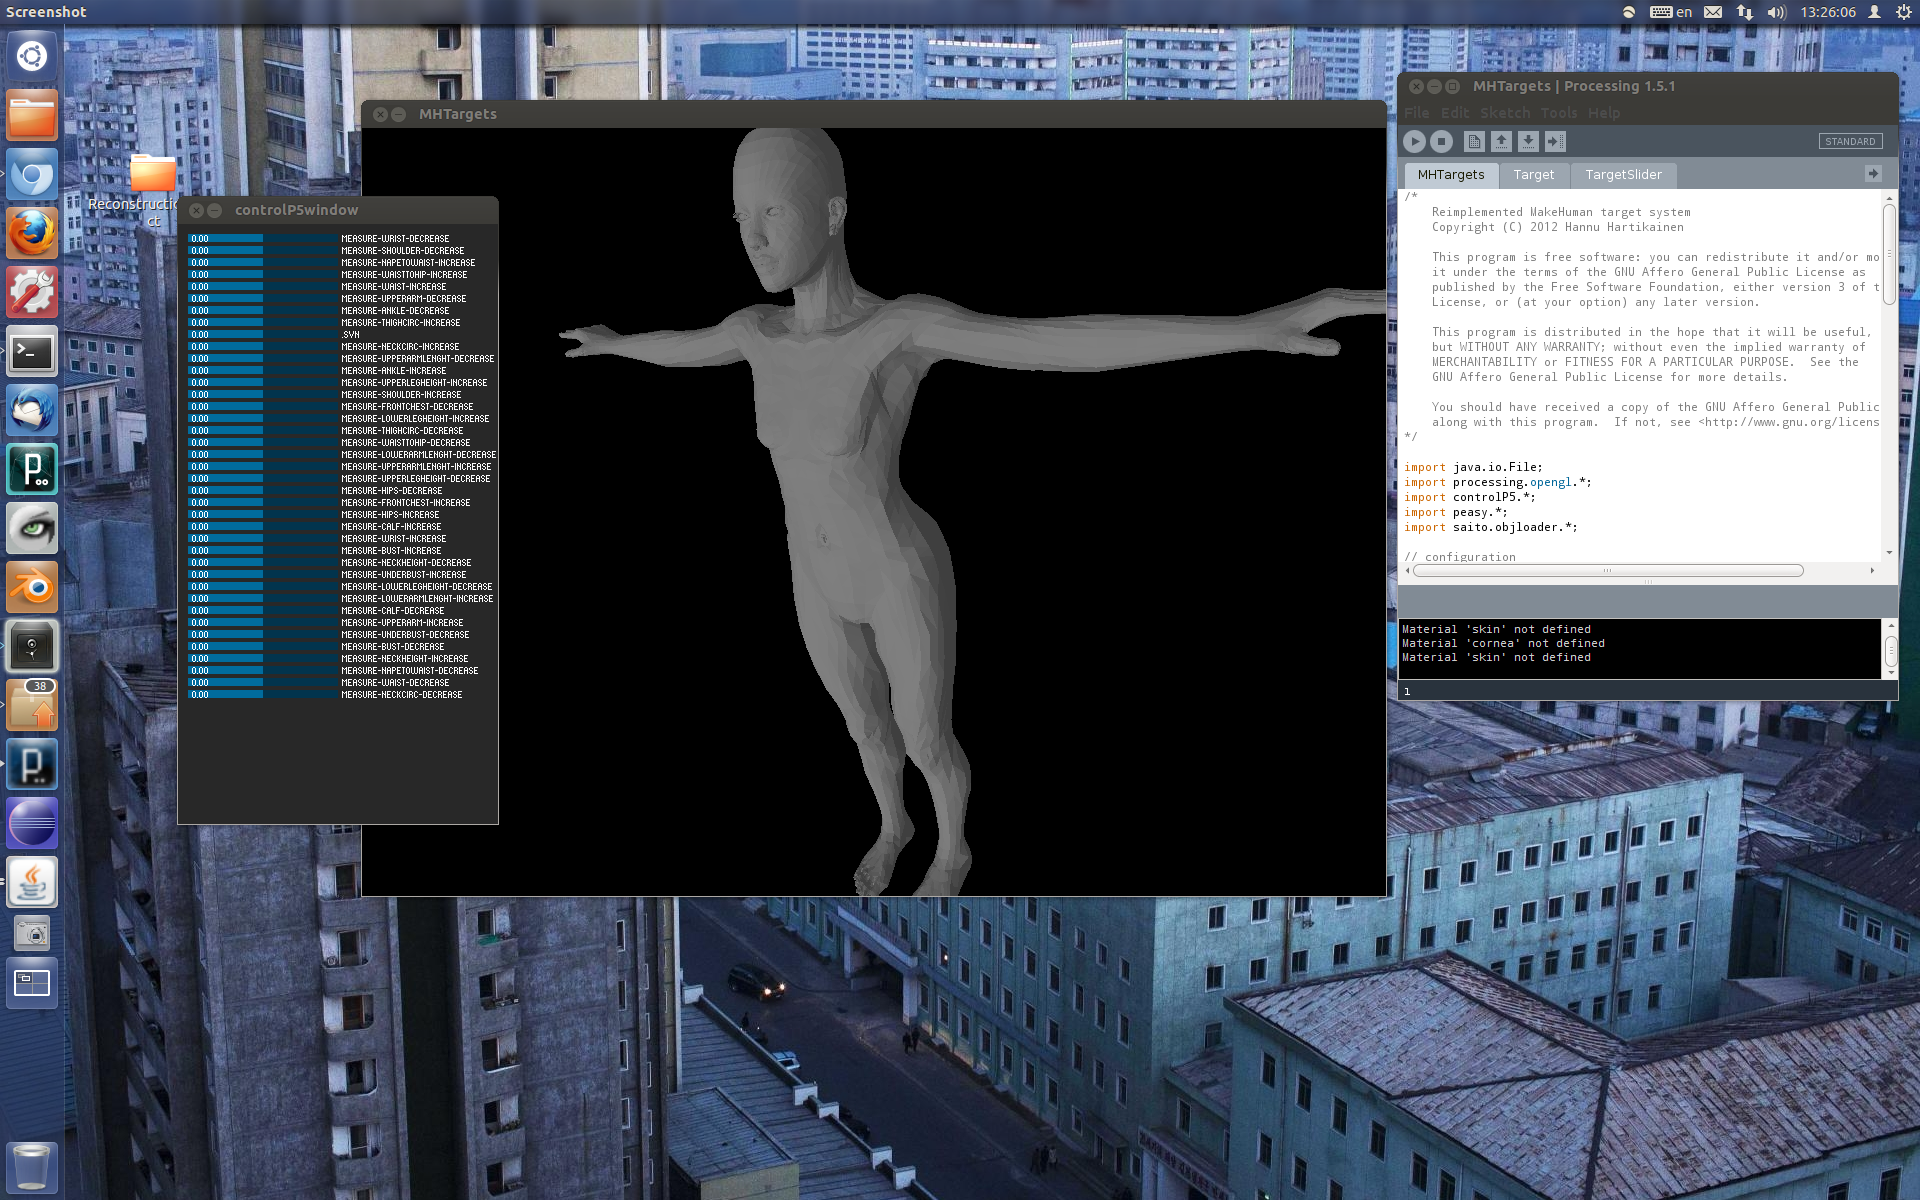
\includegraphics[width=\textwidth]{mhtargets.png}
    \caption{The reimplementation of the MakeHuman target system, showing the unmodified base mesh.}
    \label{fig:mhtargets}
\end{figure}

\begin{figure}
    \centering
    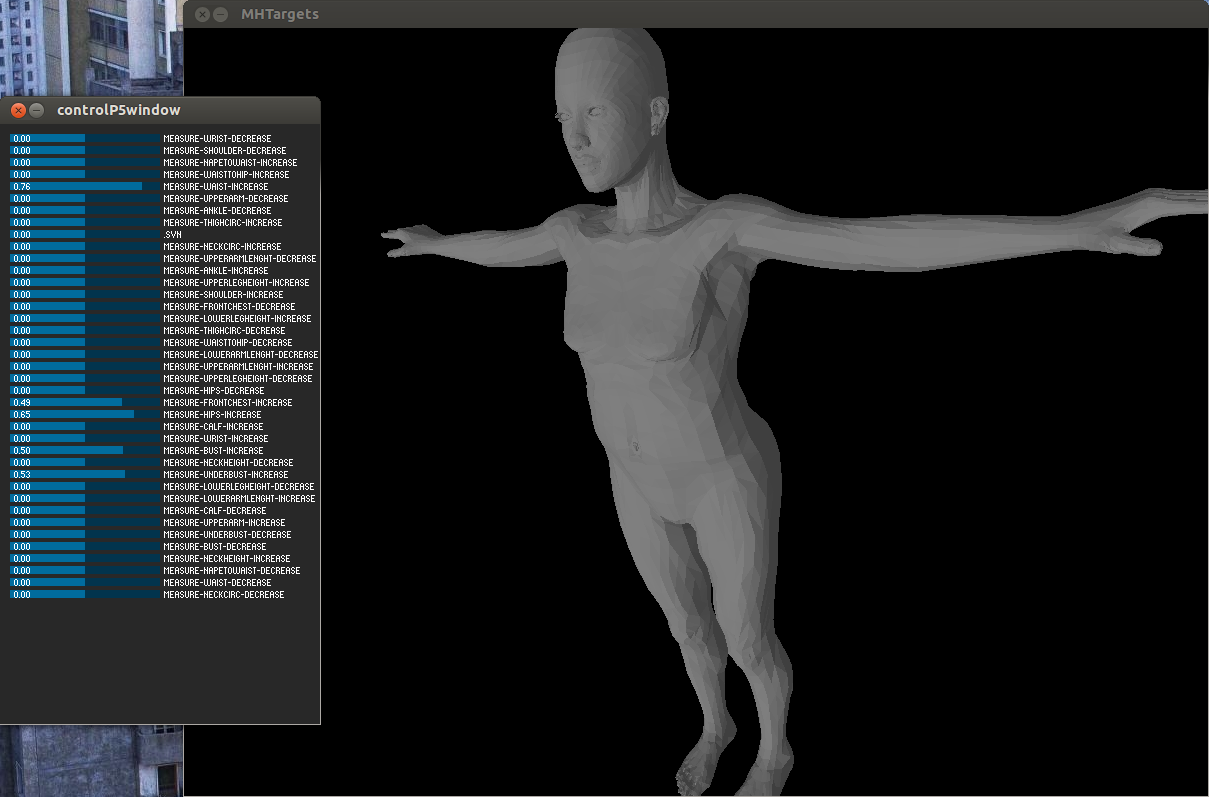
\includegraphics[width=\textwidth]{mhtargets-fat.png}
    \caption{The model in \ref{fig:mhtargets} with changed front chest, bust, underbust, waist and hip measurements.}
    \label{fig:mhtargets-fat}
\end{figure}

\section{Texturing}

\fixme{Write something here once I've done something...}


